\documentclass{beamer}

\usepackage{amsmath}

%\usetheme{}

\mode<presentation>

%Information to be included in the title page:
\title{Comparing Classical and Nonclassical Symmetries of Nonlinear Partial Differential Equations}
\author{William Helman and Daniel Sinderson}
\institute{Southern Oregon University}
\date{2023}

\begin{document}

\frame{\titlepage}
\begin{frame}
    \frametitle{Table of Contents}
    \tableofcontents
\end{frame}

\section{Introduction}
    \subsection{Project Goal}
    \subsection{What is a Symmetry?}
    \subsection{What is a Differential Equation?}
    \subsection{Background on our Equations}
\section{Results}
    \subsection{Classical Symmetries}
    \subsection{Nonclassical Symmetries}
\section{Conclusion}
    \subsection{Discussion}
    \subsection{Open Questions}
    \subsection{Next Steps}



\begin{frame}
    \frametitle{Project Goal}
    Our research objective for this project was to calculate the classical and nonclassical symmetry groups for the reduced Gibbons-Tsarev equation and the Born-Infeld equation and compare them.
\end{frame}



\begin{frame}
    \frametitle{What is a Symmetry?}
    \begin{definition}<1->
        A symmetry is a transformation that leaves an object invariant.
    \end{definition}
    \vspace*{0.5in}
    \begin{definition}<2->
        A symmetry is a change that doesn't change anything.
    \end{definition}
\end{frame}


\begin{frame}
    \frametitle{What is a Symmetry?}
    Let's see this in action using the simple linear equation $x-y=0$.\\
    \begin{center}
        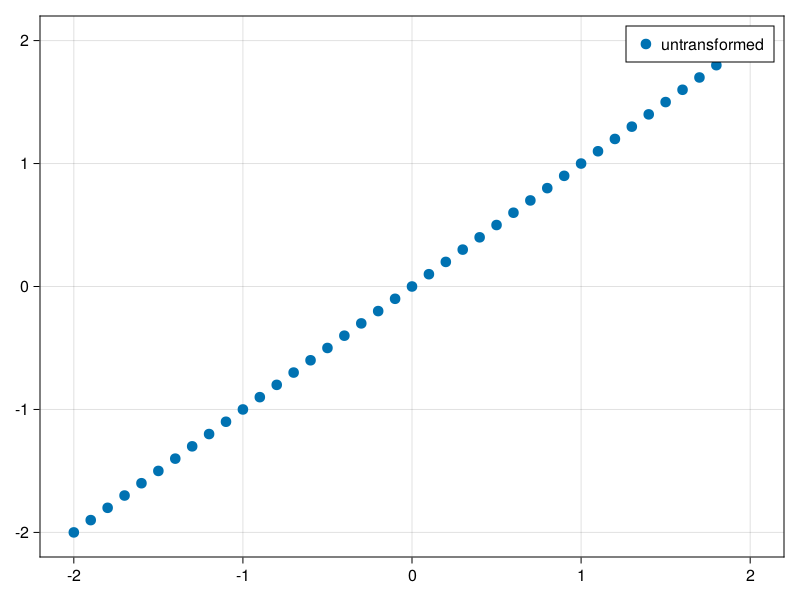
\includegraphics[width=9cm]{y=x.png}
    \end{center}
\end{frame}

\begin{frame}
    \frametitle{What is a Symmetry?}
    \begin{example}[A Non-Example]
        \begin{itemize}
            \item For our first transformation, let's define new variables\\ $\bar{x}=x+1$ and $\bar{y}=y$.
            \item Now we rewrite our equation using these new variables. \begin{equation*}
                \begin{aligned}
                    \bar{x}-\bar{y} &= 0 & \text{by definition} \\
                    x+1-y &= 0 & \text{by substitution} \\
                    y &= x+1 & \text{by rewriting in slope-intercept form}
                \end{aligned}
            \end{equation*}
            \item This transformation is not a symmetry: \\ $x-y+1\ne x-y$
        \end{itemize}        
    \end{example}
\end{frame}


\begin{frame}
    \frametitle{What is a Symmetry?}
    \framesubtitle{A Transformation that is a Symmetry}
    \begin{example}[2]<1->
        \begin{itemize}
            \item Let's define some new variables again\\ $\bar{x}=x+1$ and $\bar{y}=y+1$.
            \item Now we rewrite our equation using these new variables. \begin{equation*}
                \begin{aligned}
                    \bar{x}-\bar{y} &= 0 & \text{by definition} \\
                    (x+1)-(y+1) &= 0 & \text{by substitution} \\
                    (x-y)+(1-1) &= 0 & \text{by algebra} \\
                    x-y &= 0 & \text{by algebra} \\
                    y &= x & \text{by rewriting in slope-intercept form}
                \end{aligned}
            \end{equation*}
            \item This transformation is a symmetry: \\ $x-y = x-y$
        \end{itemize}        
    \end{example}
\end{frame}


\begin{frame}
    \frametitle{What is a Symmetry?}
    The graphs of our three equations.\\
    \begin{center}
        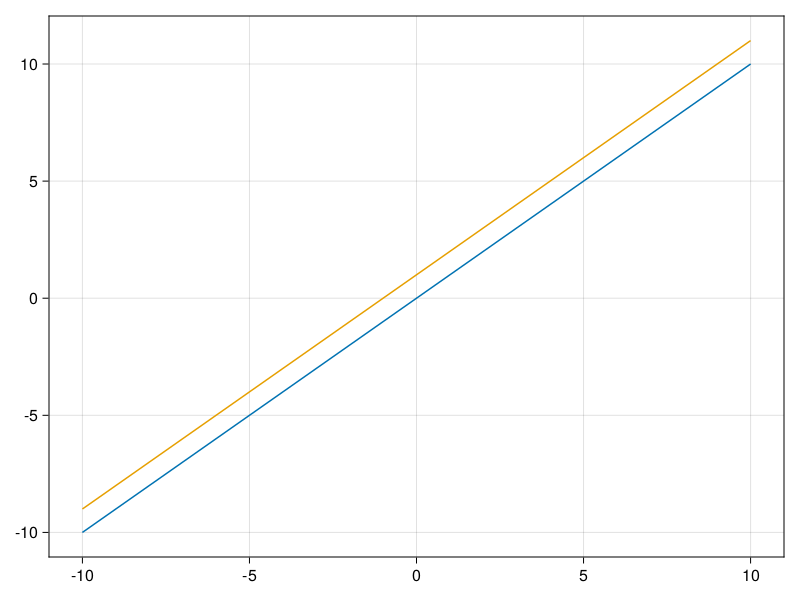
\includegraphics[width=9cm]{y=x+1.png}
    \end{center}
\end{frame}



\begin{frame}
    \frametitle{What is a Symmetry?}
    \begin{Large}
        Who cares?
    \end{Large}
    \vspace*{0.25in}
    \begin{itemize}
        \item Symmetries help us understand and solve equations that we wouldn't normally be able to.\pause
        \item Symmetries encode physically meaningful aspects of equations, like conservation laws in physics.
    \end{itemize}
\end{frame}



\begin{frame}
    \frametitle{What is a Differential Equation?}
    \begin{definition}
    \begin{itemize}
        \item A differential equation is an equation that contains both an unknown function and information about how that function relates to its rates of change. \pause
        \item Differential equations show up everywhere we model something using information about how that thing changes. This includes everything from population dynamics to planetary orbits. \pause
        \item Differential equations are different from algebraic equations, and can't be solved in the same ways.
    \end{itemize}
\end{definition}
\end{frame}



\begin{frame}
    \frametitle{What is a Differential Equation?}
    As an example, we'll use the equation for an undamped spring.\\
    \vspace*{0.125in}
    \begin{Large}
        $$m\ddot{x}=-\kappa{x}$$
    \end{Large}
    \vspace*{0.25in}
    \begin{itemize}
        \item Here $m$ is the mass, $\ddot{x}$ is the acceleration, $\kappa$ is the spring constant, and $x$ is the position.
        \item If we set both $m$ and $\kappa$ to $1$, we get $\ddot{x}=-x$.
        \item This is a simple differential equation with the algebraic solution of $x(t)=c_1\cos(t)+c_2\sin(t)$.
    \end{itemize}
\end{frame}


\begin{frame}
    \frametitle{What is a Differential Equation?}
    The graph of our spring system $x(t)=\cos(t)+\sin(t)$, where $c_1=c_2=1$.\\
    \begin{center}
        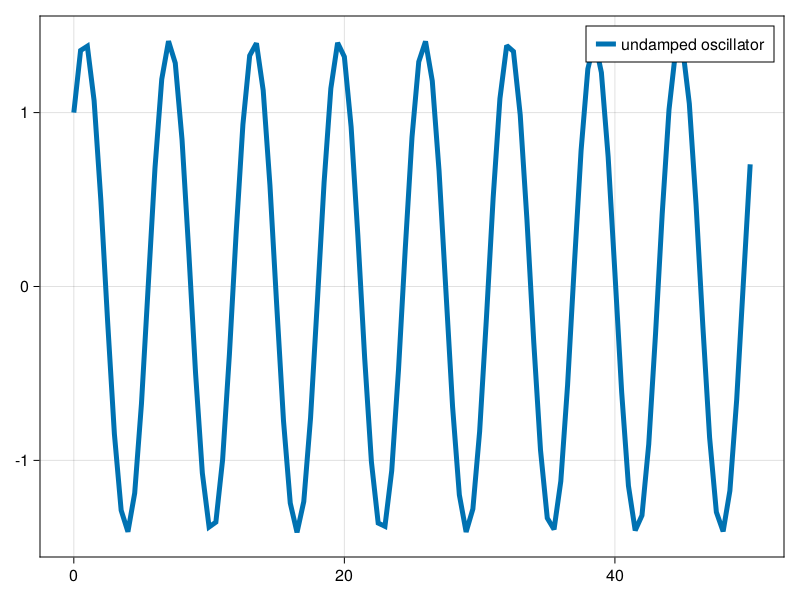
\includegraphics[width=9cm]{undamped.png}
    \end{center}
\end{frame}


\begin{frame}
    \frametitle{The History of the Born-Infeld and the reduced Gibbons-Tsarev Equations}

\end{frame}


\begin{frame}
    \frametitle{The Classical Symmetries of the Born-Infeld and the reduced Gibbons-Tsarev Equations}
    \begin{itemize}
        \item The goal of our project was to find symmetry transformations for these two PDEs, both classical and nonclassical, and compare them.
        \item It turns out that there's a standard method for calculating both kinds of symmetry transformations for differential equations.
    \end{itemize}
    \vspace*{0.125in}
    \begin{large}
        \begin{align*}
            \text{Input Equation} &\rightarrow \text{Calculate Lie's invariance condition} \\
                           &\rightarrow \text{Solve linear system of PDEs} \\
                           &\rightarrow \text{Symmetries!}
        \end{align*}
    \end{large}

\end{frame}


\begin{frame}
    \frametitle{The Classical Symmetries of the Born-Infeld and the reduced Gibbons-Tsarev Equations}
    \begin{itemize}
        \item To guarantee that a transformation is a symmetry, we need to ensure that all aspects of the equation remain the same under the transformation. \pause
        \item For a differential equation, this means that the function and any derivatives of that function that are present in the equation must not change under the transformation. \pause
        \item Lie's invariance condition gives us a way to generate transformations that meet all these requirements. \pause
        \item If you can solve Lie's invariance condition for your equation, you can find its symmetries.
    \end{itemize}
\end{frame}


\begin{frame}
    \frametitle{The Classical Symmetries of the Born-Infeld and the reduced Gibbons-Tsarev Equations}
        The general form of Lie's invariance condition is the falsely unassuming
        \vspace*{0.25in}
        \begin{Large}$$\Gamma^{(n)}\Delta |_{\Delta=0} = 0$$\end{Large}\\
        \vspace*{0.25in}
        Here $\Gamma$ is the infinitesimal operator, $n$ is the order of the equation, and $\Delta$ is the equation itself set to equal 0 (this is standard form).
\end{frame}


\begin{frame}
    \frametitle{The Classical Symmetries of the Born-Infeld and the reduced Gibbons-Tsarev Equations}
        For our equations, which are both second order PDEs in two independent variables, Lie's invariance condition looks like the following:
        \vspace*{0.25in}
        \begin{Large}$$\dots$$\end{Large}
\end{frame}


\begin{frame}
    \frametitle{The Classical Symmetries of the Born-Infeld and the reduced Gibbons-Tsarev Equations}
        \begin{itemize}
            \item The result of putting our PDEs through Lie's invariance condition was a system of $\dots$ linear PDEs for the Born-Infeld equation and $\dots$ for the reduced Gibbons-Tsarev equation. \pause
            \item Though difficult, these systems were easier to solve than the original single equations because of their linearity. This resulted in the following symmetries.
        \end{itemize}
\end{frame}


\begin{frame}
    \frametitle{The Classical Symmetries of the Born-Infeld and the reduced Gibbons-Tsarev Equations}
        \begin{large}Classical Symmetries of the Born-Infeld Equation\end{large}
        \begin{itemize}
            \item .
            \item .
            \item .
        \end{itemize}
        \vspace*{0.25in}
        \begin{large}Classical Symmetries of the reduced Gibbons-Tsarev Equation\end{large}
        \begin{itemize}
            \item .
            \item .
            \item .
        \end{itemize}
\end{frame}


\begin{frame}
    \frametitle{The Nonclassical Symmetries of the Born-Infeld and the reduced Gibbons-Tsarev Equations}

\end{frame}



\begin{frame}
    \frametitle{Future Work: Does Integrability Imply Equivalence of Classical and Nonclassical Symmetries?}

\end{frame}



\begin{frame}
    \frametitle{Future Work: Does Equivalence of Classical and Nonclassical Symmetries Imply Integrability?}

\end{frame}



\end{document}